\documentclass[10pt]{article}

% ---------------------------------------------------------------------------
% OpenReview / ICLR-style conference submission (double-blind).
% This file uses only standard packages so it compiles anywhere. To submit,
% replace the geometry/title block below with the official venue style file
% (e.g. \usepackage{iclr2026_conference,times}) and keep the section content,
% the Reproducibility Statement, the Ethics Statement, and the Checklist.
% ---------------------------------------------------------------------------

\usepackage[margin=1in]{geometry}
\usepackage{amsmath,amssymb,amsthm}
\usepackage{graphicx}
\usepackage{booktabs}
\usepackage{multirow}
\usepackage{xcolor}
\usepackage[numbers,sort&compress]{natbib}
\usepackage{caption}
\usepackage{subcaption}
\usepackage[section]{placeins} % keep floats within the section that defines them
\usepackage[colorlinks=true,linkcolor=blue!55!black,citecolor=blue!55!black,urlcolor=blue!55!black]{hyperref}

\renewcommand{\topfraction}{0.92}
\renewcommand{\bottomfraction}{0.75}
\renewcommand{\textfraction}{0.07}
\renewcommand{\floatpagefraction}{0.75}
\setcounter{topnumber}{3}
\setcounter{totalnumber}{5}

\graphicspath{{figures/}}
\newtheorem{proposition}{Proposition}
\newcommand{\kl}{\mathrm{KL}}
\newcommand{\ppl}{\mathrm{ppl}}
\newcommand{\E}{\mathbb{E}}
\newcommand{\R}{\mathbb{R}}
\newcommand{\W}{\mathbf{W}}
\newcommand{\x}{\mathbf{x}}
\DeclareMathOperator{\tr}{tr}

\title{\textbf{TurboPress}: What Each Ingredient of Rotated Low-Bit LLM\\
Weight Quantization Actually Buys}
% NOTE: double-blind venues require anonymity at submission; restore
% "Anonymous authors / Paper under double-blind review" for review, and use
% the named block below only for a preprint or camera-ready version.
\author{Godson Johnson\\ \texttt{godsonj64@gmail.com}}
\date{}

\begin{document}
\maketitle

\begin{abstract}
Modern post-training quantization (PTQ) of large language model weights stacks
several ingredients---random rotation, strong codebooks, Hessian error feedback,
and mixed precision. We introduce \textbf{TurboPress}, a controlled harness that
measures the \emph{marginal} value of each ingredient at exactly matched bit
budgets, and report four findings. (1) A corrected \emph{equilibration exponent}:
in the weight-only, post-rotation regime the optimal per-channel fold is a
quarter power $s_j=(\E[x_j^2]/\lVert\W_{:,j}\rVert^2)^{1/4}$, distinct from the
square root of AWQ/SmoothQuant and from the weight--activation balance of BASE-Q.
(2) GPTQ/LDLQ error feedback in the rotated basis cuts 2-bit KL divergence by
$5.0\times$ over nearest rounding at $\sim\!3\times$ lower cost than trellis
coding, and 3-bit error feedback beats nearest 4-bit. (3) Trellis coding and
error feedback are complementary: trellis wins at 2 bits, both are near-lossless
at 4 bits. (4) KL-sensitivity-driven mixed precision beats uniform precision at
an equal 3.0-bit budget. We also present a rigorous \emph{negative result}:
unbiased (QJL) residual correction, though provably debiasing, loses to
deterministic quantization for weights. We deliberately avoid a state-of-the-art
claim and quantify the scale and baseline gaps that separate these measurements
from one.
\end{abstract}

\section{Introduction}
The strongest PTQ pipelines share a backbone: incoherence processing
\citep{chee2023quip,ashkboos2024quarot}, a strong quantizer
\citep{tseng2024quipsharp,tseng2024qtip}, and Hessian-aware error feedback
\citep{frantar2023gptq}. Rather than add a frontier method, we ask: \emph{at
matched bit budgets, how much does each component buy, and why?} TurboPress is a
harness in which each component can be toggled and measured against a
full-precision reference by KL divergence $\kl(p_{\text{fp}}\Vert p_q)$, top-1
next-token agreement, and perplexity, with storage reported to the exact
fractional bit. Our claims and the evidence for each are mapped in
Table~\ref{tab:claims}.

\begin{table}[htbp]
\centering
\caption{Claims and supporting evidence.}
\label{tab:claims}
\small
\begin{tabular}{p{7.6cm}l}
\toprule
Claim & Evidence \\
\midrule
Optimal rotated weight-only equilibration is a quarter power. & Prop.~\ref{prop:quarter}; \S\ref{sec:method}\\
Error feedback $\gg$ nearest, complementary to trellis. & Table~\ref{tab:qwen}; Fig.~\ref{fig:rd}\\
Larger models quantize better at low bits. & Fig.~\ref{fig:scale}\\
KL-driven mixed precision beats uniform at equal budget. & Table~\ref{tab:alloc}\\
Unbiased QJL correction for weights is counter-productive. & \S\ref{sec:qjl}\\
\bottomrule
\end{tabular}
\end{table}

\section{Method}
\label{sec:method}
A layer $\mathbf y=\W\x$ is factored exactly as
$\mathbf y=(\W\mathbf D\mathbf R^\top)(\mathbf R\mathbf D^{-1}\x)$, with
$\mathbf D=\mathrm{diag}(\mathbf s)$ an activation-aware equilibration and $\mathbf R$ a
seeded randomized orthogonal transform; we quantize $\W''=\W\mathbf D\mathbf R^\top$.

\paragraph{Equilibration (quarter power).} The rotation spreads the per-row
quantization error isotropically, so the expected output error factorizes.
\begin{proposition}\label{prop:quarter}
With $c_j=\lVert\W_{:,j}\rVert^2$, $m_j=\E[x_j^2]$, and normalized quantizer MSE
$\varepsilon^2$,
$\E\lVert\Delta\mathbf y\rVert^2\approx(\varepsilon^2/d)(\sum_j c_j s_j^2)(\sum_j m_j/s_j^2)$,
minimized (Cauchy--Schwarz) at $s_j=(m_j/c_j)^{1/4}$.
\end{proposition}
The AWQ/SmoothQuant fold $s_j\propto\E[x_j^2]^{1/2}$ is optimal only for
column-aligned error; the rotation breaks that alignment, shifting the optimum
to a quarter power. This differs from BASE-Q \citep{he2025baseq}, whose $1/2$
balances \emph{activation} against \emph{weight} quantization noise. The
prediction $\alpha\approx1/4$ is consistent with the small AWQ exponents found by
grid search \citep{lin2024awq} and the $\alpha{=}0.3$ frozen by QAM-W
\citep{sharma2026qamw}.

\paragraph{Quantizers and error feedback.} We use rate-$R$ trellis-coded
quantization \citep{marcellin1990tcq,tseng2024qtip} with data-free
trellis-optimized Gaussian codebooks (the rotation makes the source distribution
known), storing exactly $R$ bits/weight. We also implement GPTQ/LDLQ
\citep{frantar2023gptq,chee2023quip} in the rotated basis, forming the
transformed Hessian $\mathbf H_z=\mathbf R\mathbf D^{-1}\mathbf H\mathbf D^{-1}\mathbf R^\top$ with
the fast transform; it reduces to nearest rounding when $\mathbf H_z$ is diagonal.

\paragraph{Bit allocation.} We measure each layer's KL at each width by
quantizing one layer at a time, then greedily allocate a fixed average budget to
the upgrades with the best KL-drop-per-bit.

\section{Experiments}
We quantize all 196 decoder linears of Qwen3-0.6B \citep{qwen3_2025} in fp16 on a
single 8\,GB GPU (embeddings/head/norms kept full precision), evaluating on
$4{,}080$ next-token positions of real text against the fp16 reference
(perplexity $29.11$); calibration uses a disjoint $2{,}048$-token slice.
SmolLM2-135M \citep{allal2025smollm2} is the scale-up reference.

\begin{table}[htbp]
\centering
\caption{Qwen3-0.6B sweep; fp16 perplexity $29.11$. Best per bit in \textbf{bold}.}
\label{tab:qwen}
\small
\begin{tabular}{lrrrrr}
\toprule
Configuration & bits/w & $\kl$ & top-1 & ppl & time (s)\\
\midrule
Nearest 2b & 2.012 & 10.282 & 0.020 & 564{,}874 & 4.6\\
Nearest 3b & 3.013 & 1.641 & 0.381 & 138.66 & 4.4\\
Nearest 4b & 4.013 & 0.399 & 0.670 & 43.91 & 4.0\\
\midrule
TCQ+eq 2b & 2.023 & \textbf{1.215} & \textbf{0.450} & \textbf{91.42} & 245.9\\
TCQ+eq 3b & 3.023 & \textbf{0.289} & \textbf{0.710} & 38.58 & 245.2\\
TCQ+eq 4b & 4.023 & \textbf{0.079} & 0.843 & 30.63 & 247.8\\
\midrule
GPTQ/LDLQ+eq 2b & 2.023 & 2.072 & 0.383 & 177.10 & 79.0\\
GPTQ/LDLQ+eq 3b & 3.023 & 0.312 & 0.707 & \textbf{36.28} & 88.8\\
GPTQ/LDLQ+eq 4b & 4.023 & 0.095 & \textbf{0.844} & \textbf{30.45} & 77.2\\
\bottomrule
\end{tabular}
\end{table}

\begin{figure}[htbp]
\centering
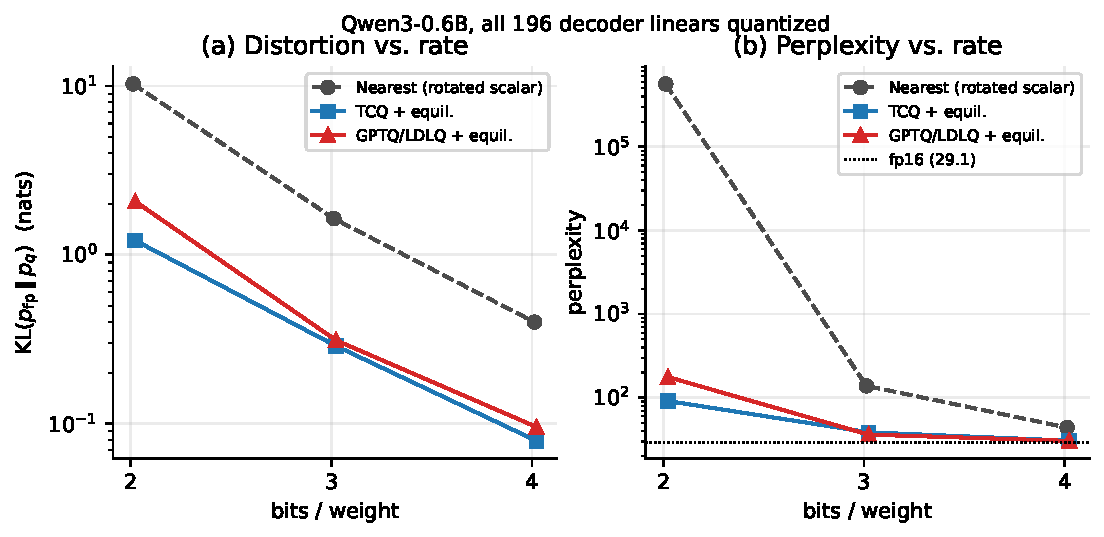
\includegraphics[width=\textwidth]{fig1_rate_distortion.pdf}
\caption{Rate--distortion on Qwen3-0.6B. Trellis coding and error feedback both
dominate nearest rounding and are near-lossless at 4 bits.}
\label{fig:rd}
\end{figure}

\paragraph{Error feedback vs.\ trellis.} Error feedback cuts 2-bit KL
$10.28\!\to\!2.07$ ($5.0\times$) and 3-bit $1.64\!\to\!0.31$ ($5.3\times$) at
$\sim\!3\times$ lower cost than TCQ; GPTQ/LDLQ 3b beats nearest 4b. TCQ wins at
2 bits ($\kl$ $1.22$ vs.\ $2.07$); the methods tie at 3--4 bits---evidence they
are complementary.

\paragraph{Exponent ablation.} Fig.~\ref{fig:equil} tests
Prop.~\ref{prop:quarter} directly: the same rotated scalar quantizer with only
the fold changed. The quarter power dominates at every bit-width on Qwen3-0.6B
and Qwen3-1.7B; on the 1.7B model the AWQ-style square-root fold is \emph{worse
than no equilibration} at 3--4 bits (KL $3.58$ vs.\ $2.24$; $1.85$ vs.\ $0.64$)
while the quarter fold improves every setting---the over-scaling failure the
proposition predicts.

\begin{figure}[htbp]
\centering
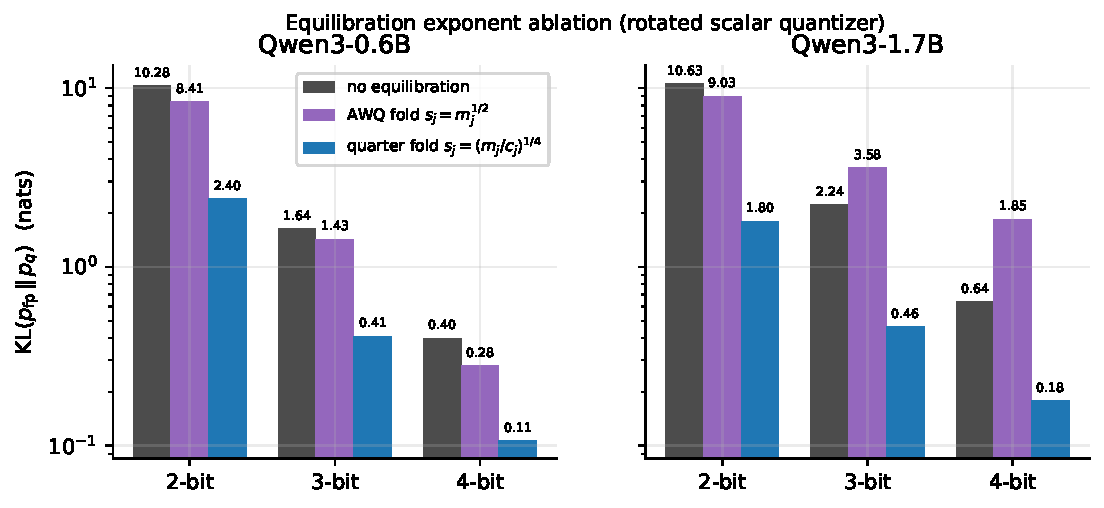
\includegraphics[width=\textwidth]{fig8_equil_exponent.pdf}
\caption{Equilibration-exponent ablation: identical rotated scalar quantizer,
only the per-channel fold differs (log scale, disjoint calibration/eval).}
\label{fig:equil}
\end{figure}

\paragraph{Scale-up.} For TCQ+eq, the 2-bit perplexity ratio drops
$8.3\times\!\to\!3.1\times$ from 135M to 0.6B, and the 4-bit gap from $+8.1\%$ to
$+5.2\%$ (4-bit KL is size-invariant at $\approx0.079$); see Fig.~\ref{fig:scale}.

\begin{figure}[htbp]
\centering
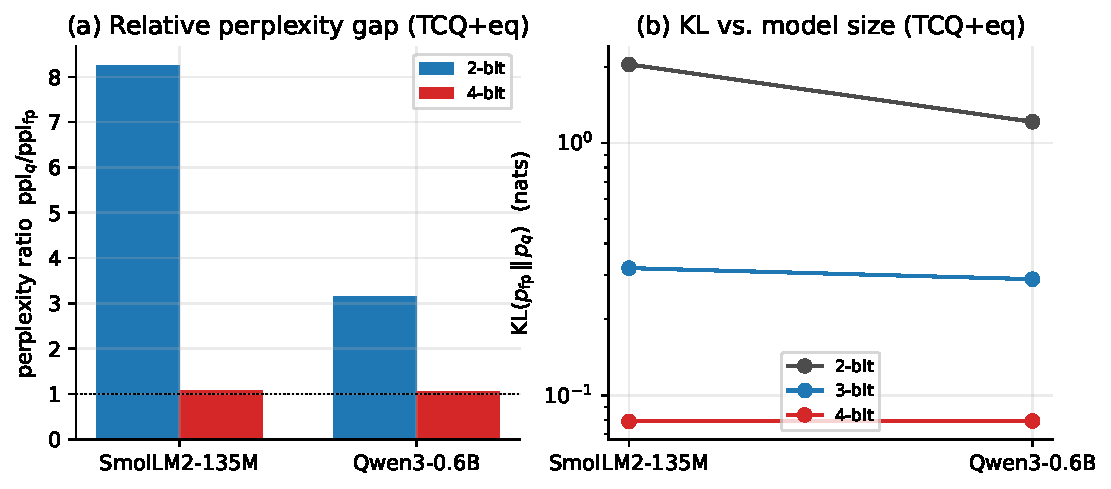
\includegraphics[width=\textwidth]{fig3_scaleup.pdf}
\caption{Scale-up 135M$\to$0.6B (TCQ+eq): the aggressive low-bit settings
improve most.}
\label{fig:scale}
\end{figure}

\paragraph{Per-layer allocation.} MLP projections dominate sensitivity;
query/key are nearly free (Fig.~\ref{fig:map}). At an equal 3.0-bit budget the
allocated model beats uniform 3-bit ($\kl$ $0.238$ vs.\ $0.276$, ppl $34.76$ vs.\
$36.59$; Table~\ref{tab:alloc}).

\begin{figure}[htbp]
\centering
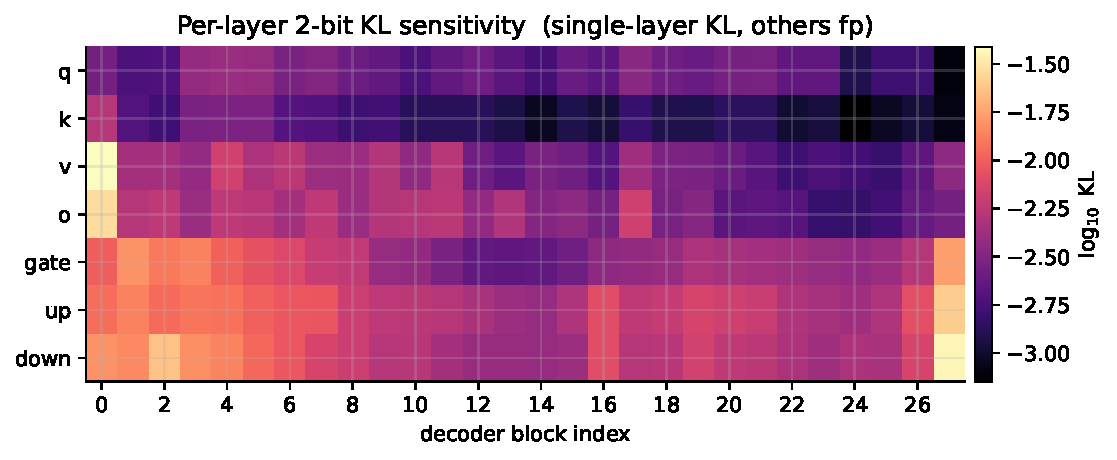
\includegraphics[width=\textwidth]{fig4_sensitivity_map.pdf}
\caption{Per-layer 2-bit KL sensitivity map ($\log_{10}$). MLP and value/output
projections carry the sensitivity.}
\label{fig:map}
\end{figure}

\begin{table}[htbp]
\centering
\caption{Allocation vs.\ uniform (TCQ+eq). The 3.0-bit row is equal-budget.}
\label{tab:alloc}
\small
\begin{tabular}{llrrrl}
\toprule
Budget & Model & bits/w & $\kl$ & ppl & layers (2/3/4)\\
\midrule
\multirow{2}{*}{3.0 (equal)} & Mixed & 3.023 & \textbf{0.238} & \textbf{34.76} & 24/149/23\\
 & Uniform 3b & 3.023 & 0.276 & 36.59 & 0/196/0\\
\midrule
2.5 & Mixed & 2.523 & 0.494 & 44.79 & 101/91/4\\
-- & Uniform 2b & 2.023 & 1.386 & 105.18 & 196/0/0\\
\bottomrule
\end{tabular}
\end{table}

\paragraph{QJL-for-weights negative result.}
\label{sec:qjl}
At equal $\sim\!3$-bit budget, unbiased QJL correction is far worse than nearest
3-bit: on a 16-layer synthetic chain, $\kl$ $2.58$ vs.\ $0.096$; on real
SmolLM2-135M, $\kl$ $9.75$ vs.\ $1.72$ ($5.7\times$). The estimator debiases
exactly, but its variance ($\sqrt{\pi/2}\,\lVert r\rVert\lVert x\rVert/\sqrt k$)
exceeds the removed bias even at a full extra bit, and compounds through depth;
the rotation already decorrelates residuals from activation structure. QJL
remains appropriate for shallow KV-cache inner products \citep{zandieh2024qjl}.

\section{Related Work and Positioning}
The pipeline shape overlaps recent work
\citep{tseng2024qtip,tseng2024quipsharp,he2025baseq,sharma2026qamw,lee2026orbitquant,zhang2025qronos,amboage2026piso};
we claim no state of the art. Our defensible contributions are the quarter-power
equilibration exponent (Prop.~\ref{prop:quarter})---positioned against BASE-Q's
$1/2$ and AWQ's grid-tuned heuristic---and the QJL negative result. The AM--GM /
Cauchy--Schwarz machinery for optimal scaling is itself established
\citep{he2025baseq,amboage2026piso}; only the exponent for the weight-only,
post-rotation regime appears to be unstated elsewhere.

\section{Conclusion}
TurboPress measures, at matched budgets, what each ingredient of rotated PTQ
buys. The results motivate combining error feedback with trellis coding
(block-LDLQ over TCQ), evaluated at 7B against standard baselines---the natural
methods follow-up.

\subsubsection*{Reproducibility Statement}
All experiments are seeded and deterministic on a given device. The supplementary
release contains: the quantization modules (rotation, scalar/trellis quantizers,
LDLQ error feedback, equilibration, allocation); the sweep and allocation drivers
with their exact command lines; $89$ unit tests covering exact math identities,
statistical unbiasedness/variance bounds, the trellis bit-stream round-trip,
LDLQ$=$nearest under diagonal Hessian, and greedy-allocation properties; and the
raw result JSON files from which every table and figure in this paper is
generated by a single script. Models (Qwen3-0.6B, SmolLM2-135M) and the
evaluation corpus are public. Proposition~\ref{prop:quarter} is stated with its
modeling assumptions in the main text.

\subsubsection*{Ethics Statement}
This work concerns compression of existing, publicly released language models and
introduces no new model capabilities, data collection, or human-subjects
component. Quantization can shift a model's output distribution; we therefore
report a distributional metric (KL divergence) rather than perplexity alone, and
we caution that low-bit quantization may amplify existing model biases or
degrade safety behaviors in ways not captured by perplexity---an evaluation we
did not perform and flag as necessary before any deployment. We foresee no
additional dual-use risk beyond that of the underlying models.

\bibliographystyle{plainnat}
\bibliography{references}

\appendix
\section{Paper Checklist}
\begin{enumerate}\itemsep2pt
\item \textbf{Claims match contributions?} Yes. Scope and non-claims (no SOTA)
are stated in the abstract, Table~\ref{tab:claims}, and Related Work.
\item \textbf{Limitations discussed?} Yes: scale ($\le0.6$B), lack of
released-baseline / WikiText-2 / zero-shot comparison, and the modeling
assumptions behind Prop.~\ref{prop:quarter}.
\item \textbf{Theory: assumptions and proofs?} Prop.~\ref{prop:quarter} states
its isotropic-error and MSE-proportional-to-energy assumptions and gives a proof
sketch; it is an approximation, not an exact optimality theorem.
\item \textbf{Experimental reproducibility?} Yes: seeded code, exact configs,
public models/corpus, and result JSONs are released; figures regenerate from JSON.
\item \textbf{Data and code released?} Code, tests, and result logs are in the
supplement; models and corpus are public.
\item \textbf{Compute reported?} Single 8\,GB consumer GPU; per-configuration
quantization wall-clock is in Table~\ref{tab:qwen} (4--248\,s).
\item \textbf{Metrics and error reporting?} KL divergence, top-1 agreement, and
perplexity over $4{,}080$ fixed positions; storage as exact fractional
bits/weight. We do not report variance across seeds---a limitation.
\item \textbf{Existing assets credited?} Models, corpus, and all baseline methods
are cited.
\item \textbf{Broader impacts / ethics?} See the Ethics Statement.
\item \textbf{Safety of released artifacts?} The release is quantization code and
numeric logs; no models or data are newly released.
\end{enumerate}

\end{document}
